\documentclass[12pt]{article}
\usepackage[czech]{babel}
\usepackage[utf8]{inputenc} 
\usepackage{listings}
\lstset{language=C}
\usepackage{minted}
\usepackage[hidelinks]{hyperref}
\usepackage{graphicx}
\usepackage{caption}
\usepackage[all]{hypcap}
\usepackage{pdfpages}

\newcommand{\Csh}{C\#}

\renewcommand\listingscaption{Výpis}


\begin{document}
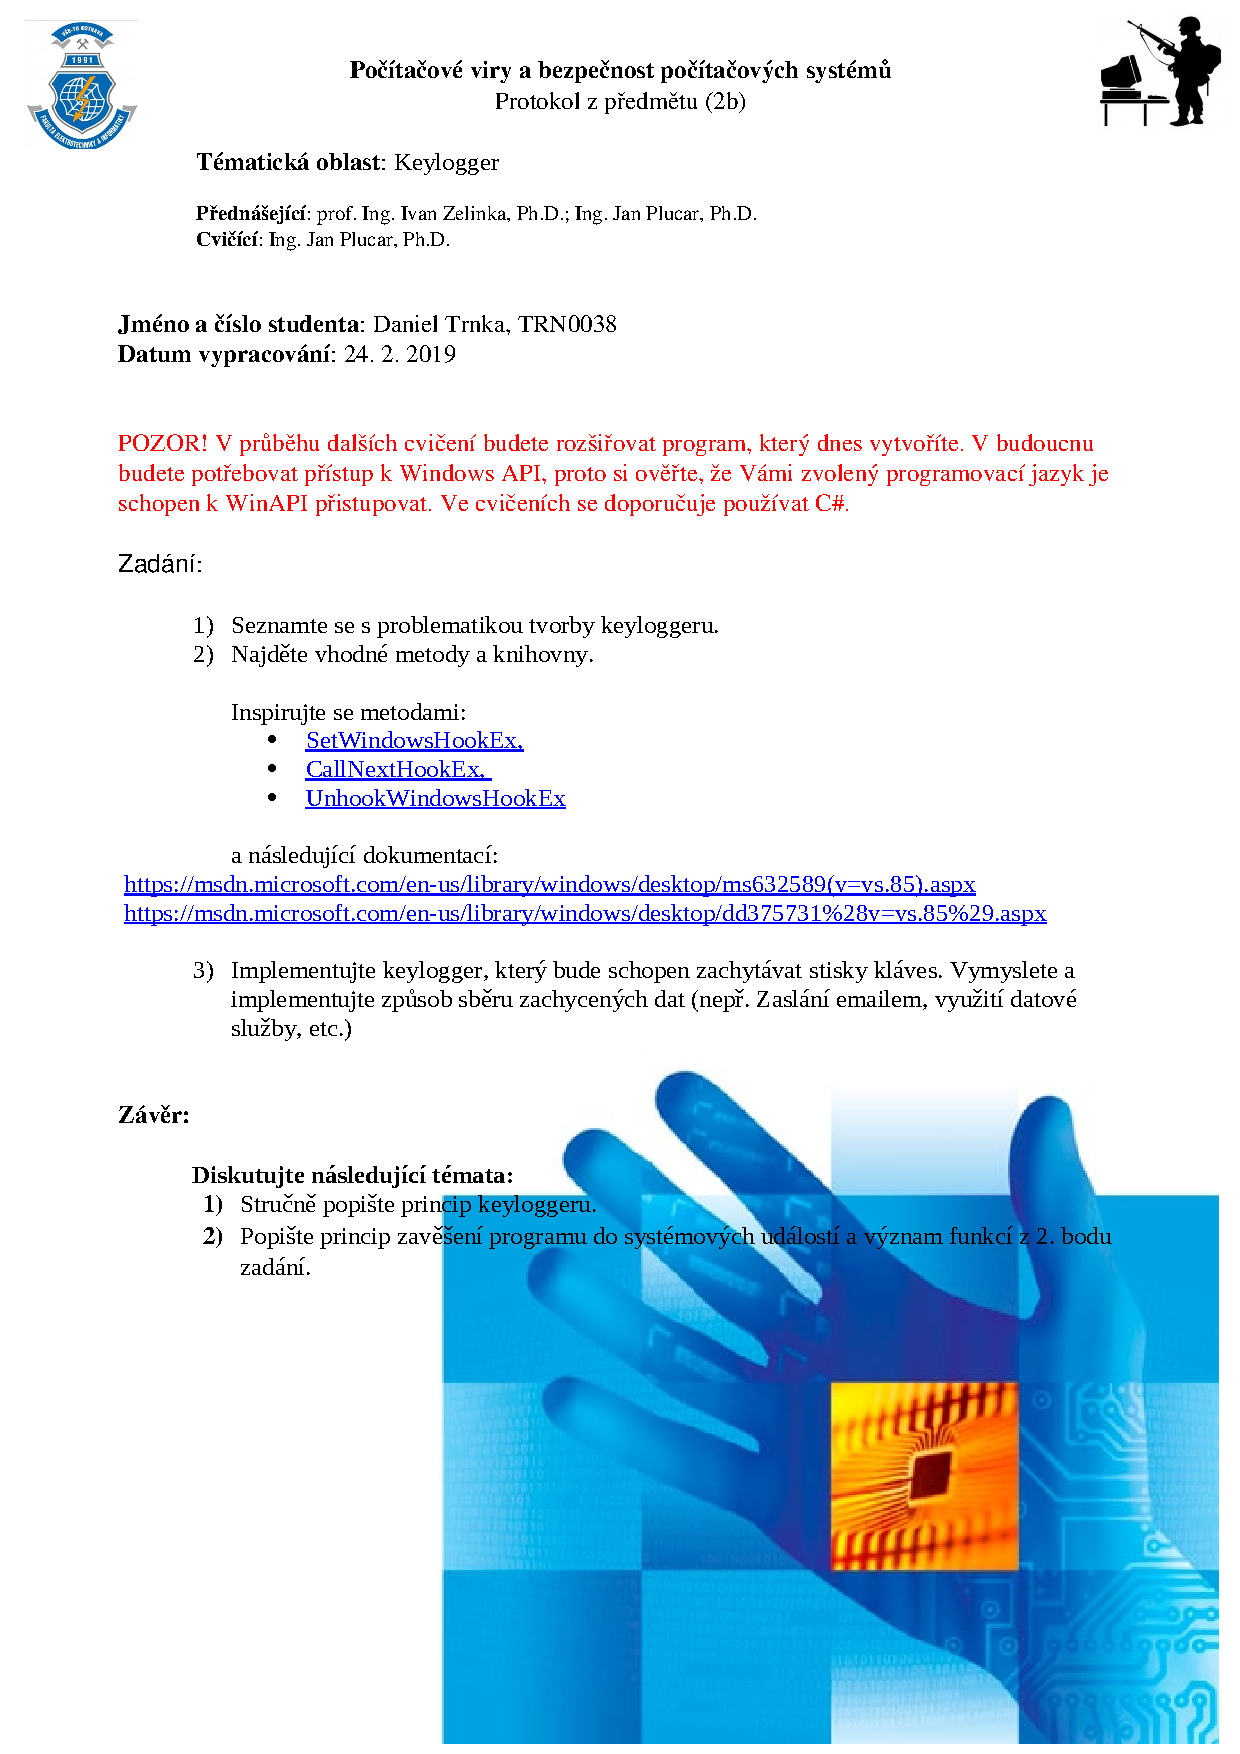
\includepdf[pages=1]{zadani.pdf}

\textit{Keylogger} je program zachytávající stisky kláves, které následně ukládá či posílá pryč z počítače oběti.
Někdy se však může jednat i o legitimní činnost, kdy se sbírají data o používaní aplikace, které slouží k jejímu následnému vylepšení.


Systém Windows zasílá události jako stisk kláves do aktivních (focused) aplikací pomocí zpráv.
Pro funkční příjem zpráv je zapotřebí vytvořit okno a číst zprávy pomocí funkce \mintinline{c}{GetMessage(...)}.

Abychom byli schopní číst všechny stisknuté klávesy tak si musíme zaregistrovat tzv. \textit{hook}, který se provede ještě před tím než se zpráva doručí do aktivního okna.
Pro zachytávání události na klávesnici existují dva typy hooks - \textit{WH\_KEYBOARD} a \textit{WH\_KEYBOARD\_LL}.
Hook \textit{WH\_KEYBOARD\_LL} lze použít i bez okna - je však nutné zavolat funkci \mintinline{c}{GetMessage(...)}.
Proces v této funkci zůstane (funkce se neopustí, protože nikdy nepřijde žádná zpráva) a zajistí volání callback hooku.

Callback pro daný hook se registruje pomocí funkce \mintinline{c}{SetWindowsHookExA(...)} z dynamické knihovny \textit{user32.dll}:

\begin{minted}{c++}
HHOOK SetWindowsHookExA(
	int       idHook,
	HOOKPROC  lpfn,
	HINSTANCE hmod,
	DWORD     dwThreadId
);
\end{minted}

Funkce vrací identifikátor zaregistrovaného hooku (je to \mintinline{c}{void**}) pro jeho možnou pozdější odregistrací pomocí \mintinline{c}{UnhookWindowsHookEx(HHOOK hook)}.
Prvním argumentem je typ hooku.
Konstanta \textit{WH\_KEYBOARD\_LL} je 13.
Dalším argumentem je ukazatel na funkci typu: 
\mint{c}|LRESULT(int code, WPARAM wParam, LPARAM lParam)|
Další dva parametry nemají pro \textit{WH\_KEYBOARD\_LL} využití a jsou nastaveny na nulovou hodnotu.

První argument callbacku uvádí, zda se má provést jeho obsluha.
Další argument typu \mintinline{c}{unsigned int} značí událost klávesnice jako \mintinline{c}{WM_KEYDOWN} a \mintinline{c}{WM_KEYUP}.
Posledním argumentem je ukazatel na strukturu \mintinline{c}{KBDLLHOOKSTRUCT*}.
\begin{minipage}{\textwidth}
\begin{minted}{c}
struct KBDLLHOOKSTRUCT {
	DWORD     vkCode;
	DWORD     scanCode;
	DWORD     flags;
	DWORD     time;
	ULONG_PTR dwExtraInfo;
}
\end{minted}
\end{minipage}

Struktura obsahuje identifikaci stisknuté klávesy  \mintinline{c}{vkCode}\footnote{\url{https://docs.microsoft.com/en-us/windows/desktop/inputdev/virtual-key-codes}} a také  \mintinline{c}{scanCode}, který je identifikaci pro konkrétní klávesnici.
Hodnota \mintinline{c}{vkCode} označuje klávesu, bez ohledu na nastaveném layoutu klávesnice či zmáčknutého \mbox{\textsc{Shift/Caps Lock}}.
Pro zjištění, který znak byl skutečně zadán lze použít funkci \mintinline{c}{ToAscii(...)}:
\begin{minted}{c}
int ToAscii(
	UINT       uVirtKey,
	UINT       uScanCode,
	const BYTE *lpKeyState,
	LPWORD     lpChar,
	UINT       uFlags
);
\end{minted}

Funkce očekává v prvních dvou argumentech \mintinline{c}{vkCode} a \mintinline{c}{scanCode}.
V dalším argumentu očekává pole o velikosti 255 bajtů, která značí stav stisknutých kláves dle značení virtual-key.
Pokud je klavesa stisknutá tak je na odpovídajícím indexu nastaven nejvyšší bit - hexadecimálně \textit{0x80}.
Pokud je zapnutý \textsc{Caps Lock}, tak je nastaveny nejnižší bit.

Aby fungoval správně převod na velká/malá písmena tak bylo nutné nastavit klávesu \mintinline{c}{VK_SHIFT} při stisknutí levého nebo pravého \textsc{Shift}.

Do argumentu \mintinline{c}{lpChar} funkce uloží maximálně dva znaky.
Dva znaky jsou navráceny pokud uživatel zadal klávesu pro diakritické znaménko a neplatný znak. Platná kombinace vytvoří znak \textit{ó}, neplatná dva znaky: \textit{´f}.

Pro univerzalní keylogger by bylo vhodnější použít alternativní funkci \mintinline{c}{ToUnicode(...)}.

Callback musí zavolat \mintinline{c}{CallNextHookEx}, jinak by nedošlo k provedení hooku v jiné aplikaci.
Pokud bychom danou funkci nezavolali a vrátili 0, tak se další aplikace nedozví o stisknuté klávese.
Dále je také nutné podotknout, že obsluha nesmí být blokující a trvat dlouho, jinak ostatní aplikace budou dostávat události opožděně.

Další alternativou je použití funkce \mintinline{c}{SHORT GetAsyncKeyState(int vKey)}, kdy aplikace testuje všechny požadované virt keys. 
Řešení pak vede k busy waiting, kdy se procesorový čas spotřebovává jen na kontrolu, zda nedošlo ke stisku klávesy.
Další nevýhodou je, že funkce vrací pouze informaci, zda byla klávesa zmáčknuta od posledního zavolání - tudíž nejsme schopní zjistit počet opakovaných stisku jedné klávesy.


{
	\inputminted{c}{../c/simple.c}
	\captionof{listing}{Zachytávání kláves pomocí hooku v C}
	\label{lst:simple_c}
}


Z uvedené ukázky ve výpisu \ref{lst:simple_c} je vidět, že přístup k Windows API v~jazyce~C je jednoduchý - deklarace funkci a konstant jsou v hlavičkových souborech a knihovna \textit{user32.dll} je přilinkována.
Použití v jazyce \Csh{} bez externích knihoven se mírně komplikuje, protože se musí uvedena dynamická knihovna \textit{user32.dll} do procesu v době běhu namapovat a následně získat ukazatele na dané funkce.
Dále je nutné si vytvořit i konstanty.

Pro zpřístupnění funkce z DLL se vytvoří funkce se stejným názvem a klíčovým slovem extern, které značí, že implementace bude dodána později.
Dále se k dané funkci přidá atribut \textit{DllImport}, ve kterém se uvede dynamická knihovna obsahující požadovaný symbol:


\begin{minted}{csharp}
delegate IntPtr LowLevelKeyboardProc(
	int nCode,
	IntPtr wParam,
	IntPtr lParam
);

[DllImport("user32.dll", CharSet = CharSet.Auto, SetLastError = true)]
public static extern IntPtr SetWindowsHookEx(
	int idHook,
	LowLevelKeyboardProc lpfn,
	IntPtr hMod,
	uint dwThreadId
);
\end{minted}

Získat data ze struktury \mintinline{c}{KBDLLHOOKSTRUCT} lze například pomocí \mintinline{c}{Marshal}.
První dva argumenty struktury jsou 32bitové čísla, které lze získat pomocí: 
\begin{minted}{C}
int vkCode = Marshal.ReadInt32(lParam);
int scanCode = Marshal.ReadInt32(lParam, 4);
\end{minted}

Dalším zádrhelem je, že životnost proměnné s callbackem hook funkce musí být po celou dobu, kdy je hook zaregistrován.
V opačném případě se proměnná uvolní garbage collectorem nebo ji nahradí jiná data na stacku, čímž pak může hook skočit do neplatné funkce.

Protože hook funkce nesmí trvat dlouho, tak se jednotlivé znaky přidávají do fronty odkud si je vybírá vlákno a posílá pomocí ICMPv6 Echo Request nebo pomocí HTTP POST požadavku.

Zachycený ASCII text je převeden do hexadecimálního formátu a vložen do spodních 64 bitů IPv6 sítě 2001:470:5816:f::/64 (viz obrázek~\ref{fig:ip}). Je zde místo až pro 8 znaků.
Na vytvořenou adresu je následně odeslán ICMP echo-request paket.

Síť 2001:470:5816::/48 je nasměrovaná na router, který má ve směrovací tabulce záznam, aby pakety do sítě 2001:470:5816:f::/64 směroval dále na Raspberry Pi, na kterém lze jednoduše zachytávat přijaté pakety (výpis~\ref{lst:awk}) pomocí programu \textit{tcpdump} a následně extrahovat pomocí \textit{awk} znaky s ukládáním do souboru dle zdrojové IPv6 adresy.
Zaznamenaný text lze jednoduše sledovat pomocí:

\begin{minted}{bash}
$ tail -f /tmp/keylogger/2001\:470\:5816\:0\:78d2\:8e8d\:e526\:580a
facebook.comuser@example.comya3EeJai7zee9ch
\end{minted}



\begin{figure}
\centering
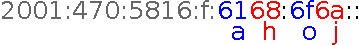
\includegraphics{ip.pdf}
\caption{Uložení znaků do IPv6 adresy}
\label{fig:ip}
\end{figure}


Raspberry Pi ještě obsahuje routovací záznam, aby odpovídal na ICMP echo požadavky z celé sítě: \mint{bash}|route add local 2001:470:5816:f::/64 dev lo|

\begin{listing}[ht]
\inputminted{bash}{../capture.sh}
\caption{Skript pro sběr zachycených znaků z ICMP echo request paketů}
\label{lst:awk}
\end{listing}

Keylogger byl označený jako podezřelý pouze u 10 antivirů z 61:

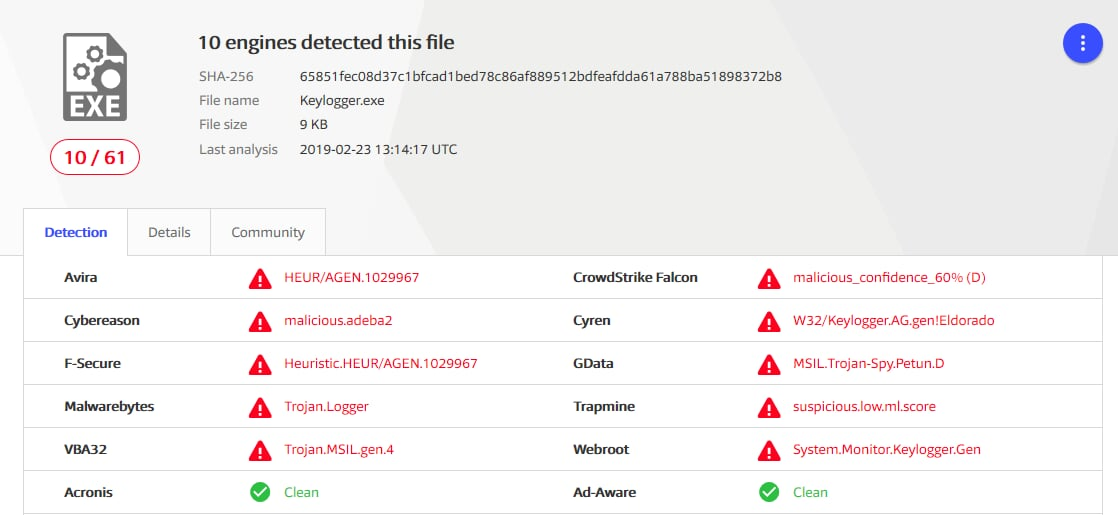
\includegraphics[width=\textwidth]{virustotal}

Alternativně lze také posílat zachycené klávesy přes HTTPS a ideálně server umístit například za CloudFlare, čímž se může ztížit hledání podezřelého sítového provozu, protože dnes velká spousta webu využívá CloudFlare.
Před zahájením HTTPS komunikace však klient posílá hostname (SNI) v čitelné podobě, který lze v provozu detekovat.
Do nedávna bylo možné využít Domain Fronting, kdy se v SNI uvedl nějaký legitimní hostname a poté v zašifrované HTTP hlavičce se uvedl hostname pro zlomyslný web.



\end{document}